\newpage
\vspace{6cm}
\section{IMPLEMENTATION}
\hspace{0.7cm}In this project, our group chose Python to implement the system because it is easy when working with raw socket. We just need to import libraries and use existed methods. Below is the general working mechanism of our system including both client side and server side:

\begin{figure}[h]
\centering
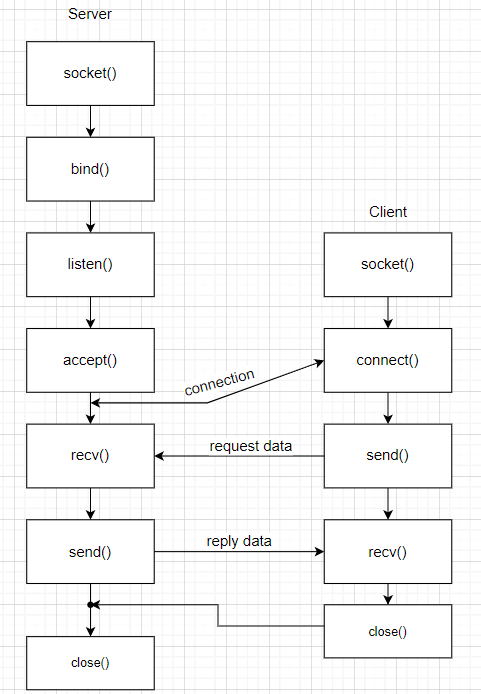
\includegraphics{images/socket.png}
\end{figure}

\newpage
\underline{\textbf{* Note: }}
\begin{itemize}
    \item \textbf{Socket(): }create socket
    \item \textbf{Bind(): }  associate a socket with an IP address and a port number
    \item \textbf{Listen(): } tell a socket to listen for incoming connections
    \item \textbf{Accept(): } accept an incoming connection on a listening socket
    \item \textbf{Connect(): }connect a socket to a server
    \item \textbf{Recv():}  receive data on a socket
    \item \textbf{Send(): }send data out over a socket
    \item \textbf{Close(): }close a socket descriptor
\end{itemize}

\hspace{0.7cm}The server must be run first. In either side, the initial step is to create a socket. Then, the server has to associate its socket with an IP address and a port number, and wait for incoming connections. Meanwhile, after creating a socket, the client asks to connect its socket to the server. If the server accepts the connection, the client will be able to send data over the socket. In case the server receives the data, it will send back a corresponding message to the client. This data transfer process can be repeated until the socket descriptor is closed. In this last step, it has to be sure that the socket from the client must be closed before the one from the server to avoid the interference.
